\documentclass[10pt,conference,compsocconf]{IEEEtran}

\usepackage[hidelinks]{hyperref}
\usepackage{graphicx}	% For figure environment
\usepackage{amsmath}
\usepackage{caption}
\usepackage{subcaption}
\usepackage[
 disable
]{todonotes}
\usepackage{float}

% \usepackage[dvipsnames]{xcolor}
\definecolor{io}{HTML}{23445D}
\definecolor{conv}{HTML}{6C8EBF}
\definecolor{batchnorm}{HTML}{82B366}
\definecolor{relu}{HTML}{F8A197}
\definecolor{sigmoid}{HTML}{B46504}
\definecolor{convtransp}{HTML}{9673A6}
\definecolor{add}{HTML}{666666}
\definecolor{maxpool}{HTML}{0E8088}
\definecolor{concat}{HTML}{D6B656}

\begin{document}
\title{Detecting Roads in Aerial Images using Deep Neural Networks}
\author{
  Karim Assi\\
  \texttt{karim.assi@epfl.ch}
  \and
  Alexandre Pinazza\\
  \texttt{alexandre.pinazza@epfl.ch}
  \and
  Milan Reljin\\
  \texttt{milan.reljin@epfl.ch}
}

\maketitle

%\begin{abstract}
    
%\end{abstract}

\section{Introduction}

This study deals with the segmentation of aerial images: our goal is to accurately determine whether each image pixel is a road or a background. In literature, convolutional neural networks have been shown to be effective in solving this task. We implement a model following a U-Net architecture that outperforms more basic approaches and accurately segments unseen data. 

\section{U-Net Encoder-Decoder}

\subsection{Model description}

\begin{figure*}
    \centering
    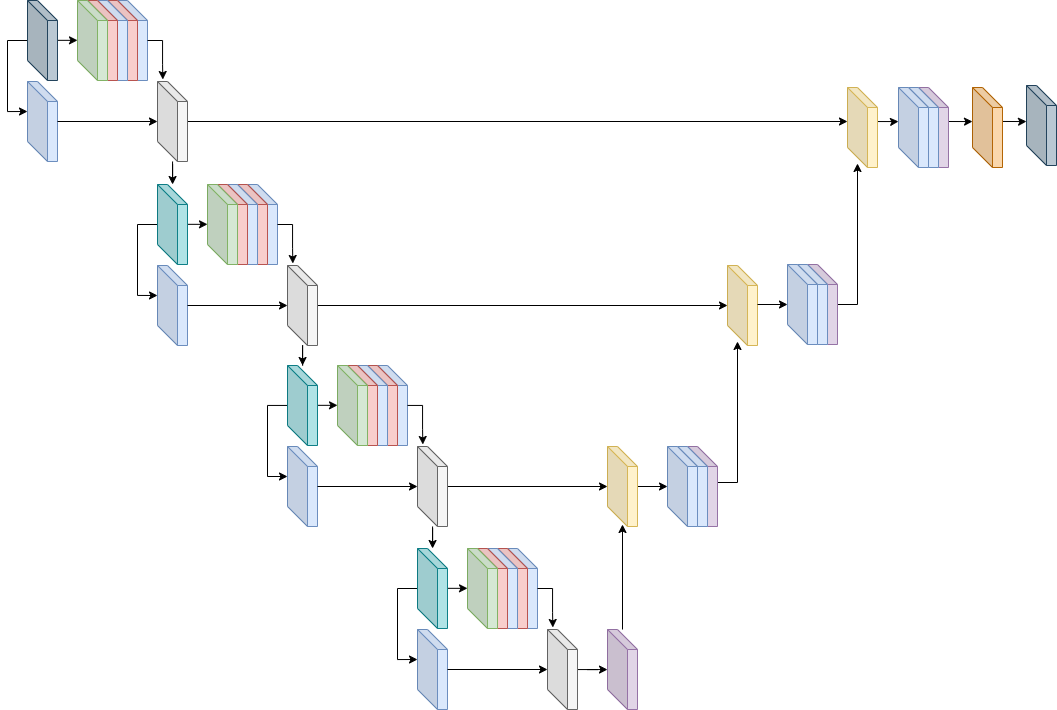
\includegraphics[width = 0.8 \textwidth, height = 0.4 \textwidth]{doc/images/Unet.png}
    \caption{Structural description of our network. Legend: 
    \textcolor{conv}{Convolution},
    \textcolor{convtransp}{Transposed convolution},
    \textcolor{maxpool}{Max pooling},
    \textcolor{batchnorm}{Batch normalization},
    \textcolor{relu}{ReLu}, \textcolor{sigmoid}{Sigmoid},
    \textcolor{io}{Input and output}, \textcolor{add}{Addition} (light gray), \textcolor{concat}{Concatenation}.}
    \label{fig:model_arch}
\end{figure*}

The model we propose is described by Alshaikhli et. al \cite{unet_roadseg}, an extension of the original U-Net architecture \cite{unet_medical}, and is specifically developed for road segmentation of aerial images. In this model, contraction blocks are augmented with batch normalization layers and implemented as residual blocks.  \\ 

The U-Net architecture was developed for biomedical image segmentation \cite{unet_medical}. It's a type of encoder-decoder network consisting of two parts: a contracting path and an expansive path. The contracting path is made up of several applications of convolutional layers followed by max-pool layers to extract feature vectors at different levels. The decoder part consists of several expansion blocks. Each block is made up of an up-sampling layer and a convolution layer. Up-sampling is implemented using a transposed convolution, which has the advantage of being learnable. In addition, at each level, the input to the expansion block is concatenated with the feature vector of the corresponding contraction layer. \\

The complete architecture of our model is depicted in figure \ref{fig:model_arch}. Each convolutional layer has a kernel size of $3 \times 3$, a  stride of 1 and the same padding. The first convolutional layer has 64 filters: this number is doubled in each consecutive layer of the network's encoder (left part of figure \ref{fig:model_arch}). Consequently, the decoder section applies convolutions of size 512, 256, 128 and 64 respectively. In order to add together the input of each contracting (residual) block and its output we first apply a convolution to the input in order match their dimensionality. At the end of each block, max-pooling with a kernel size of $2 \times 2$ and stride 2 is applied to down-sample the output. A transposed convolution with a kernel size of $3 \times 3$ and stride 2 is used in the decoder part (right section of figure \ref{fig:model_arch}) to up-sample the images. The final prediction is obtained using a $1 \times 1$ convolution layer followed by a sigmoid activation function. \\

During training, neural networks are updated layer by layer, while assuming that previous layers do not change. In practice, all layers are changed simultaneously, and the distribution of each layer’s inputs changes during training: this effect is known as internal covariate shift. The model uses \textit{batch normalization}, i.e. the standardization of the activations of each layer, to reduce the said effect \cite{batchnorm}. \\

Moreover, as neural networks get deeper and more complex, optimizing them becomes more difficult to the point where they get outperformed by shallower, simpler counterpart models \cite{deep_residual_nn}. This is due to a vanishing or exploding gradient. To counter this, \cite{deep_residual_nn} makes use of \textit{residual blocks} which add shortcut connections that skip one or more layers. This results in easier network optimization, because training of some layers can be avoided.

\subsection{Dataset}

Our dataset consists of satellite images acquired from Google Maps along with their ground truth equivalent (except for the testing set). The training set contains a hundred annotated aerial images, while the testing set contains fifty non-annotated images. \\

In order to remove the implicit ordering of classes introduced by integer labeling, we have represented the ground-truth images using one-hot encoding. Each ground truth image has two channels, the first one represents road pixels and the second background ones.

\subsection{Data augmentation}

As training a neural network requires a large amount of data, we first looked into ways to generate more images from the existing ones. To that end we extracted $224 \times 224$ patches with a stride value of 64 and increased our training set's size by a factor of 9. Some cities have road networks that form repetitive shapes or grids, and our model should be invariant to transformations. To account for this, we rotated each image by $15, -10, 45, -60, -78$ degrees and applied shearing transformations on both coordinates with the following shearing angles: $(15, 20), (10, 30), (30, -17), (-3, 20), (-5, -10)$, where the first angle (\textit{resp.} second) corresponds to a horizontal (\textit{resp.} vertical) shear. The data augmentation step leaves us with a total of $9'900$ images.

\section{Training the model}

We trained our model using the PyTorch framework \cite{pytorch} on Google's Colab infrastructure to make use of freely available GPUs. We reserved 20\% of the training images to serve as a validation set. 

\subsection{Choice of learning rate}
\label{sec:choice_lr}

To estimate the optimal learning rate, we performed the \emph{LR range test}  \cite{lr_estimation}. This consists in training our network starting with a low learning rate that exponentially increases with the number of iterations and then plotting the loss as a function of the learning rate: the optimal learning rate range corresponds to the point on the graph with the fastest decrease in the loss. We used the implementation of \cite{pytorch_lr_finder} to optimize the choice of the learning rate. Figure \ref{fig:lr_finder_plot} shows the resulting plot.

\begin{figure}[ht]
    \centering
    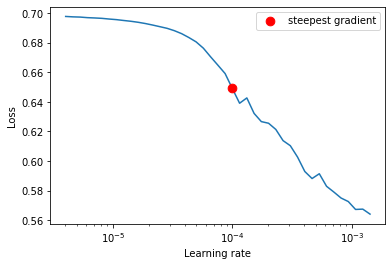
\includegraphics[width=0.6\linewidth]{doc/images/lr_finder_plot.png}
    \caption{Output plot of the LR finder used with Adam and BCE loss.}
    \label{fig:lr_finder_plot}
\end{figure}

\subsection{Choice of evaluation metric and loss function}

Our classifier should be able to recognize roads from background pixels in an aerial image. Such images typically contain more background than roads: the total area of roads can be small, compared to the picture size. Standard accuracy is therefore not a good metric, as a classifier always predicting a background would score very high. The Jaccard index, also known as the Intersection over Union score (IoU), is defined as the ratio between the intersection size of the prediction and target data over the size of their union: $J(y, \hat{y}) = \frac{|y \cap \hat{y}|}{|y \cup \hat{y}|}$. This metric takes into account the aforementioned issue and is therefore more relevant for semantic segmentation tasks \cite{reitsam_2020}. As it is preferable to have multiple metrics to assess a model, we chose to use the IoU score along with the accuracy and F1-score\footnote{Note that we used the Dice coefficient here, which represents the same metric as the F1-score.}. \\

The loss function choice has a direct influence on the training of our model, and thus has to be done carefully. Many loss functions have been used in literature on semantic segmentation \cite{loss_functions} for different types of data. The \emph{default}, and most commonly used, loss function for segmentation tasks is Binary Cross Entropy (BCE): it uses probability distributions and increases as the predicted probability diverges from the actual label. In the case of skewed data, it can weight positive examples by some coefficient. The Dice Loss, based on the Dice coefficient that is used to compute similarity between images, is also an efficient way to evaluate the segmentation of skewed data. \\

Under similar conditions, the models trained using Adam and each of the two loss functions seem to perform better using BCE than with Dice according to the metrics chosen earlier (see figure \ref{fig:loss_metrics}). For this reason we chose to continue with BCE loss. Moreover as it is provided by the Pytorch package, it means it is optimized and more stable than the Dice loss we implemented ourselves.  

\begin{figure}[ht]
    \centering
    \begin{subfigure}{0.31\linewidth}
        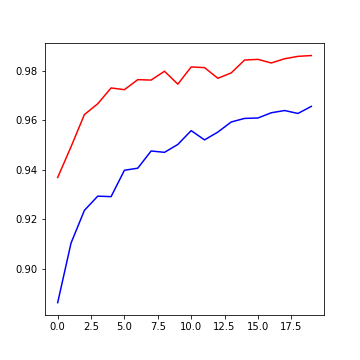
\includegraphics[width=\linewidth]{doc/images/accuracies.png}
        \caption{Accuracies}
    \end{subfigure}
    \begin{subfigure}{0.31\linewidth}
        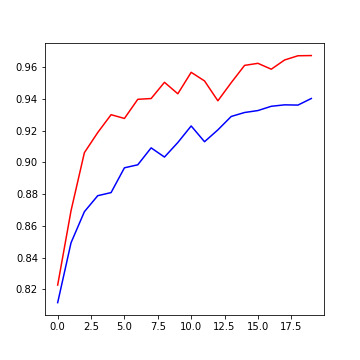
\includegraphics[width=\linewidth]{doc/images/F1_scores.png}
        \caption{F1-scores}
    \end{subfigure}
    \begin{subfigure}{0.31\linewidth}
        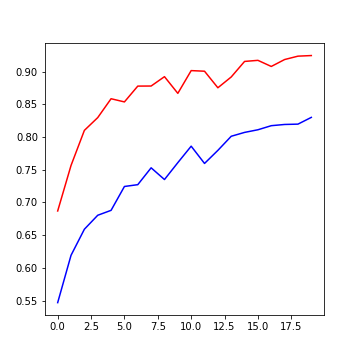
\includegraphics[width=\linewidth]{doc/images/IoU_scores.png}
        \caption{IoU-scores}
    \end{subfigure}    
    \caption{Evolution of evaluation metrics with the number of epochs, for each loss function. Legend : \textcolor{red}{BCE}, \textcolor{blue}{Dice}.}
    \label{fig:loss_metrics}
\end{figure}

\subsection{Choice of optimizer}

Choosing the optimization algorithm boils down to the choice between gradient descent (or its variants) and adaptive learning methods \cite{optimization_algorithms}. While adaptive methods (e.g. Adam) are popular in training deep neural networks, they have shown to be outperformed by SGD \cite{wilson2018marginal} with momentum and learning rate decay. SGD usually succeeds to find a minimum but takes longer to converge, and relies on a robust initialization: it may get stuck in saddle points instead of local minima. Adam on the other hand will converge much faster, but the resulting model risks not generalizing to unseen data \cite{wilson2018marginal}. \\

Momentum can help guide SGD in the relevant direction and dampen oscillations by adding a fraction $\gamma$ of the previous update vector to the current one. Values close to 1, typically $\gamma = 0.9$, are chosen in most cases \cite{optimization_algorithms, momentumvalue}. We tried both optimizers: SGD with a momentum of $0.9$ and an exponential learning rate decay of $0.95$, and Adam. In both cases, we picked an initial learning rate using the technique explained in section \ref{sec:choice_lr}. Figure \ref{fig:opt_metrics} shows the evolution of the evaluations metrics depending on the optimizer used. \\

Adam converged after 80 epochs with a final training loss of about 15 while SGD converged after 80 with a final training loss of 20. Moreover the evaluation metrics on our validation set were better when Adam converged. Based on this experiment we decided to continue with the Adam optimizer.

% starting lr for SGD  : 5e-2   training loss after 51 epochs : 21.622
% starting lr for Adam : 1e-4   training loss after 50 epochs : 22.177

\begin{figure}[ht]
    \centering
    \begin{subfigure}{0.31\linewidth}
        \centering
        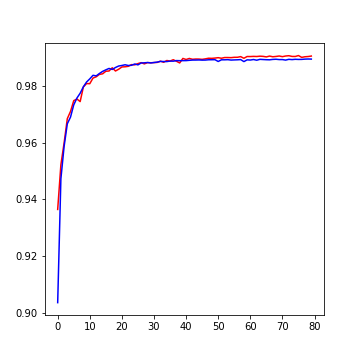
\includegraphics[width=\linewidth]{doc/images/opt_accuracies.png}
        \caption{Accuracies}
    \end{subfigure}
    \begin{subfigure}{0.31\linewidth}
        \centering
        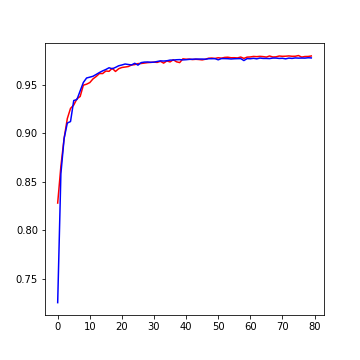
\includegraphics[width=\linewidth]{doc/images/opt_f1_scores.png}
        \caption{F1-scores}
    \end{subfigure}
    \begin{subfigure}{0.31\linewidth}
        \centering
        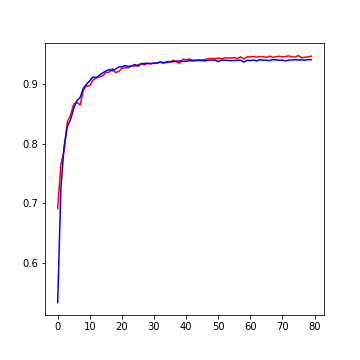
\includegraphics[width=\linewidth]{doc/images/opt_iou_scores.png}
        \caption{IoU-scores}
    \end{subfigure}
    \caption{Evolution of the evaluation metrics for each optimizer. Legend: \textcolor{red}{Adam}, \textcolor{blue}{SGD with momentum and learning rate decay}.}
    \label{fig:opt_metrics}
\end{figure}

\section{Evaluation}

To assess our model, we need to have a baseline model to which we can compare our model's performance. During training, we reserved 20\% of the training set to serve as a local validation set, on which we report the metrics in the following sections.\\

To that extent, we implemented a Convolutional Neural Network based on the provided one. It consists of two convolutional and pooling layers with a binary cross entropy loss. Its structure is shown in table \ref{tab:cnn_struct}. It works on $16 \times 16$ image patches and predicts whether each patch represents a road or not. In the training set, a patch was classified as a road if more than $25\%$ percent of its pixels were road pixels. We used the same threshold as the one used to generate the submission files from a mask. The performance of our baseline model is shown in table \ref{tab:cnn-perf} for different optimizers. We trained the model until the training loss converged. Notice that the setting using SGD with momentum and learning rate decay converged faster than the one using Adam; this confirms the claim that adaptive methods are not always advantageous \cite{wilson2018marginal}.

\begin{table}[ht]
    \centering
    \begin{tabular}{|c|c|c|}
        \hline
        Layer & Kernel size     & Output size  \\ \hline
        \textit{input} & -               & $16 \times 16 \times 3$\\ \hline
        \textit{conv1} & $5 \times 5$    & $16 \times 16 \times 32$ \\ \hline
        \textit{pool1} & $2 \times 2$    & $6 \times 6 \times 32 $\\ \hline
        \textit{conv2} & $3 \times 3$    & $ 4 \times 4 \times 64$ \\ \hline
        \textit{pool2} & $2 \times 2$    & $2 \times 2 \times 64$ \\ \hline
        \textit{fc1}   & $2 \times 2$    & $1 \times 1 \times 512$ \\ \hline
        \textit{fc2}   & $1 \times 1$    & $1$ \\ \hline
    \end{tabular}
    \caption{Structure of baseline CNN}
    \label{tab:cnn_struct}
\end{table}

\begin{table}[ht]
    \centering
    \begin{tabular}{|c|c|c|c|c|c|c|}
    \hline
        Ep.     & LR        & LR decay & Optim.     & Loss & Accuracy & F1      \\ \hline \hline
        200     & $0.0013$  & -        & Adam       & BCE  & 0.828   & 0.670   \\ \hline % Training loss: ~ 1000 DONE
        140     & $0.1$     & 0.95     & SGD.       & BCE  & 0.841   & 0.672   \\ \hline % Training loss: ~ 399 Done
        
    \end{tabular}
    \caption{Performance evaluation of baseline CNN under different parameters. For the SGD optimizer, we set a momentum of 0.9 and an exponential LR decay. The LR values are found using the technique previously mentioned.}
    \label{tab:cnn-perf}
\end{table}

\begin{figure*}[ht]
    \centering
    
    \begin{subfigure}{0.20\textwidth}
        \centering
        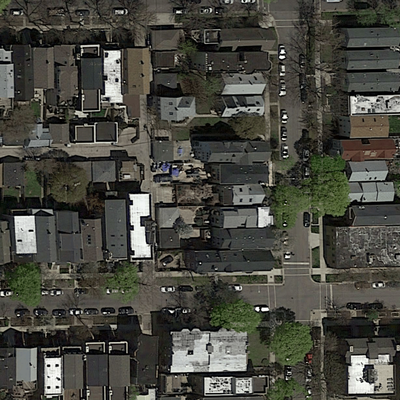
\includegraphics[width=0.9\linewidth]{doc/images/perfect_input.png}
    \end{subfigure}
    \begin{subfigure}{0.20\linewidth}
        \centering
        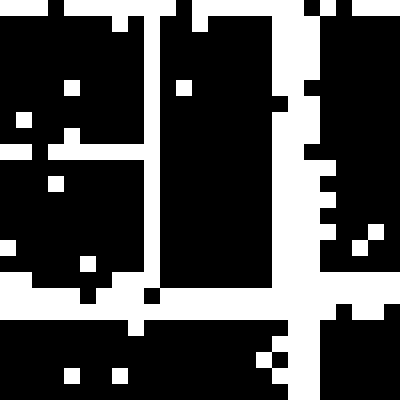
\includegraphics[width=0.9\linewidth]{doc/images/perfect_cnn.png}
    \end{subfigure}
    \begin{subfigure}{0.20\linewidth}
        \centering
        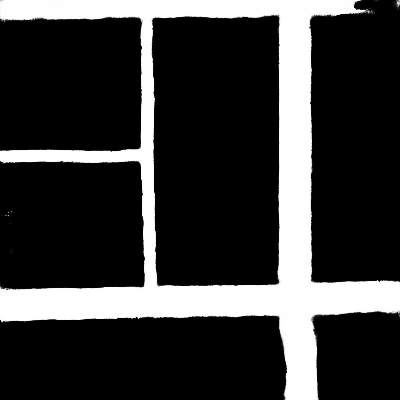
\includegraphics[width=0.9\linewidth]{doc/images/perfect_unet.png}
    \end{subfigure}
    \begin{subfigure}{0.20\linewidth}
        \centering
        
\includegraphics[width=0.9\linewidth]{doc/images/perfect_gt.png}
    \end{subfigure}\\
    
    \vspace{0.5cm}
    
    \begin{subfigure}{0.20\textwidth}
        \centering
        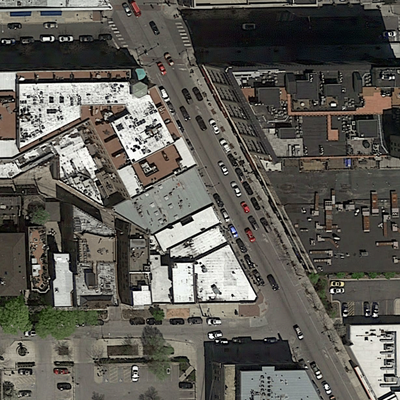
\includegraphics[width=0.9\linewidth]{doc/images/shadow_input.png}
    \end{subfigure}
    \begin{subfigure}{0.20\linewidth}
        \centering
        
\includegraphics[width=0.9\linewidth]{doc/images/shadow_cnn.png}
    \end{subfigure}
    \begin{subfigure}{0.20\linewidth}
        \centering
        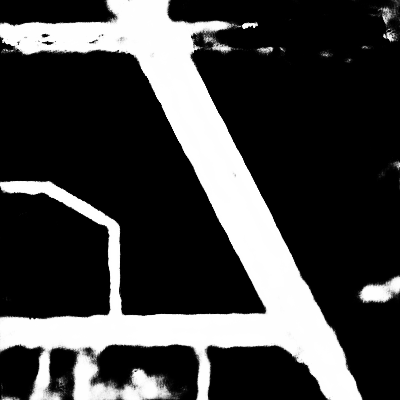
\includegraphics[width=0.9\linewidth]{doc/images/shadow_unet.png}
    \end{subfigure}
    \begin{subfigure}{0.20\linewidth}
        \centering
        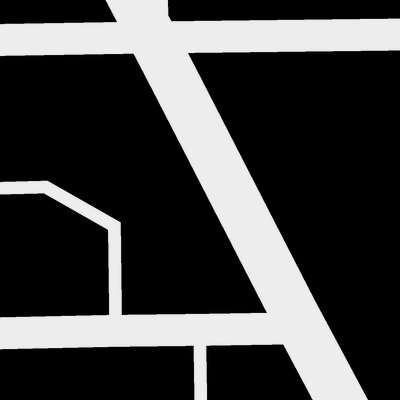
\includegraphics[width=0.9\linewidth]{doc/images/shadow_gt.png}
    \end{subfigure}

    \caption{Prediction of our model compared to the baseline model and the ground truth. From left to right: original image, output of CNN, output of our model (U-Net), ground truth.}
    \label{fig:output_comparison}
\end{figure*}

\section{Results}

The baseline CNN model has an accuracy of 84\% and an F1-score of 0.67 on a local validation set, while our U-Net model achieves an accuracy of 99\%, an F1-score of 0.98 and an Jaccard index of 0.95. As our model is fully convolutional with 3 max-pooling layers, it accepts any RGB image having dimensions being multiples of 8: this is handy as we can directly feed a whole image of the testing set. Figure \ref{fig:output_comparison} shows a prediction of our models for two different images. 

\section{Further work}

\subsection{Better data augmentation}
In our data augmentation phase, we only applied the transformation once and with fixed values. While this increases the number of images and makes the resulting model slightly transformation-invariant, it can only learn the images for these particular transformations and not for arbitrary ones. To fix that, we could use random transformations and apply them on the fly, each time we retrieve an image from our dataset. This forces the model to be invariant to transformations as it will most likely never see the same transformed image twice in the training set. Moreover, we noticed that our model often fails at recognizing roads shadowed by large buildings and houses. An example of this effect is shown in the second row of figure \ref{fig:output_comparison}. To account for that, we could augment the data by randomly modifying brightness, contrast and saturation to train the model to be invariant to color and lighting variations.    

\subsection{Post-processing}
Mnih and Hinton \cite{post_processing} have shown that they achieved a substantial improvement in predictive performance by using local spatial coherence: if one pixel is a road then it is likely that neighboring ones are roads. This technique could also improve our model as it sometimes output blurry masks (see figure \ref{fig:blurry_output}).
\begin{figure}[ht]
    \centering
    \begin{subfigure}{0.45\linewidth}
        \centering
        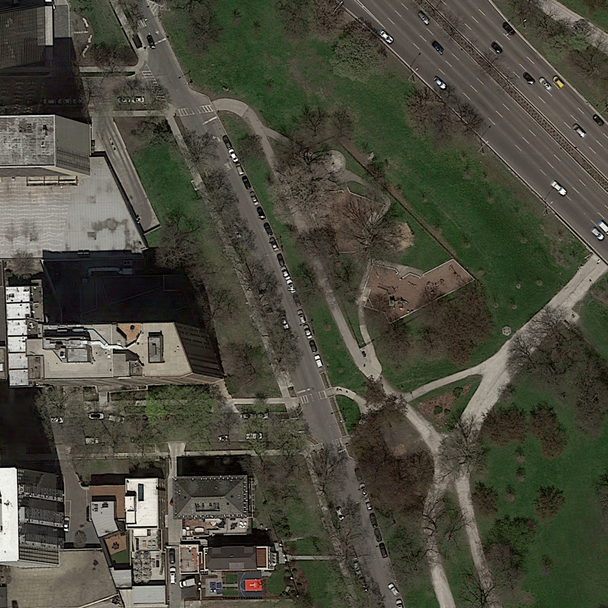
\includegraphics[width=0.65\linewidth]{doc/images/blurry_input.png}
        \caption{Input image}
    \end{subfigure}
    \begin{subfigure}{0.45\linewidth}
        \centering
        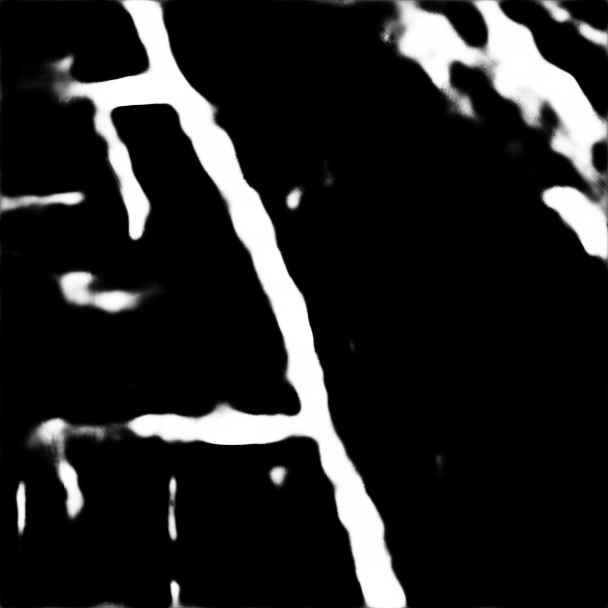
\includegraphics[width=0.65\linewidth]{images/blurry_output.png}
        \caption{Prediction of our model}
    \end{subfigure}
    \caption{Blurry output of our model}
    \label{fig:blurry_output}
\end{figure}

\subsection{Transfer learning}

So far, training our model took a few hours with a relatively small dataset, in comparison with \emph{ImageNet} that has more that 14 millions images. It could have been beneficial to use a well trained and tested model, tweak it, and use it to our advantage. Such pre-trained models are trained on very large datasets for a long time.

\section{Conclusion}

We implemented a classifier based on the U-Net architecture that can correctly and accurately segment roads from aerial images. That model can be further improved by focusing more on pre-processing and post-processing, or by looking into transfer learning. Nevertheless, it performs better than a basic CNN network trained under similar conditions.

\clearpage

% TODO before submission

\todo{Cleanup code}
\todo{Move metrics from training.py to separate file}
\todo{Make run.py}
\todo{Prepare README.md}


\listoftodos

\bibliographystyle{IEEEtran}
\bibliography{literature}
\nocite{*}

\end{document}
